\documentclass[a4paper,11pt]{ltjsarticle}
\usepackage[dvipdfmx]{graphicx}
\usepackage{color}
\usepackage{amssymb}
\usepackage{here}
\usepackage{subcaption}
\usepackage{amsmath}
\usepackage{listings}
\usepackage{url}

\lstset{
	%プログラム言語(複数の言語に対応,C,C++も可)
	language = Matlab,
	%背景色と透過度
	backgroundcolor={\color[gray]{.90}},
	%枠外に行った時の自動改行
	breaklines = true,
	%自動改行後のインデント量(デフォルトでは20[pt])	
	breakindent = 10pt,
	%標準の書体
	basicstyle = \ttfamily\scriptsize,
	%コメントの書体
	commentstyle = {\itshape \color[cmyk]{1,0.4,1,0}},
	%関数名等の色の設定
	classoffset = 0,
	%キーワード(int, ifなど)の書体
	keywordstyle = {\bfseries \color[cmyk]{0,1,0,0}},
	%表示する文字の書体
	stringstyle = {\ttfamily \color[rgb]{0,0,1}},
	%枠 "t"は上に線を記載, "T"は上に二重線を記載
 %他オプション:leftline,topline,bottomline,lines,single,shadowbox
	frame = TBrl,
	%frameまでの間隔(行番号とプログラムの間)
	framesep = 5pt,
	%行番号の位置
	numbers = left,
 %行番号の間隔
	stepnumber = 1,
 %行番号の書体
	numberstyle = \tiny,
 %タブの大きさ
	tabsize = 4,
	%キャプションの場所("tb"ならば上下両方に記載)
	captionpos = t
}
\begin{document}

\title{レポート課題(1) \\ 信号処理Ⅰ}

\author{学籍番号:2022531033 氏名:関川謙人}
\date{提出日:\today}
\maketitle

\section{課題1}
問題1-1:
Report1\_kadai1.mを完成させレポートに添付せよ。

解答:
課題1-1のファイルのソースコードを以下に示す。
またRMSE関数はmyRMSEとして定義し、自作した。
\lstinputlisting[title={Report1\_kadai1.m}]{DSP1/Report1_kadai1.m}

\newpage

問題1-2:入力信号、離散フーリエ変換と高速フーリエ変換により得られた
振幅スペクトルをそれぞれ図示せよ。

解答:
以下に結果を示す。
%横に3枚の画像(jpg/png)表示
\begin{figure}[H]
\begin{center}
\begin{tabular}{c}
\begin{minipage}{0.33\hsize}
\begin{center}
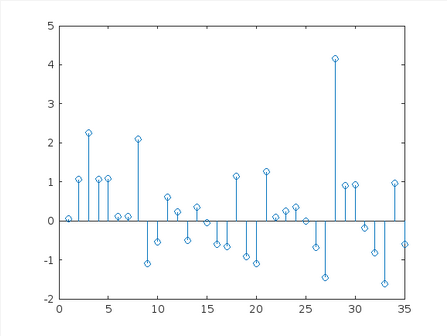
\includegraphics[width=5cm]{DSP1/r1_k1_1.png}
\end{center}
\caption{入力信号}
\label{input_signal}
\end{minipage}
\begin{minipage}{0.33\hsize}
\begin{center}
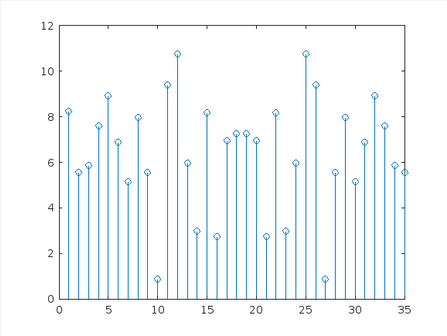
\includegraphics[width=5cm]{DSP1/r1_k1_2.png}
\end{center}
\caption{離散フーリエ変換}
\label{risan_signal}
\end{minipage}
\begin{minipage}{0.33\hsize}
\begin{center}
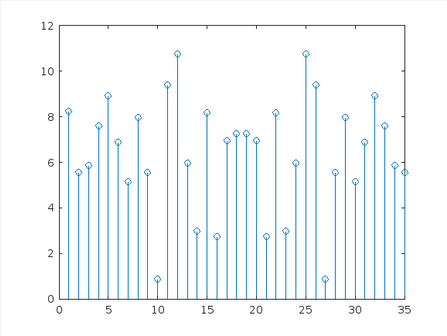
\includegraphics[width=5cm]{DSP1/r1_k1_3.png}
\end{center}
\caption{高速フーリエ変換}
\label{rapid_signal}
\end{minipage}
\end{tabular}
\end{center}
\end{figure}

問題1-3:
RMSEを算出した結果、出力結果は
\begin{lstlisting}
	4.8041e-15 - 3.9315e-15i
\end{lstlisting}
となった。すなわち
\begin{equation*}
	\mathrm{RMSE} = 4.81 \times 10^{-15} - 3.93 \times 10^{-15}i
\end{equation*}
ということになる。かなり小さい値になったため、高速フーリエ変換と離散フーリエ変換の結果は
ほぼ同じであると言える。

応用課題:
信号をプロットする際、plot関数とstem関数を用いることができる。これらの関数の出力の違いについて簡潔に説明せよ。
また、plot関数の問題点について言及せよ。

解答:
plot関数とstem関数の違いは、plot関数はxの値に対応するYのデータをプロットするのに対し、stem関数はx軸を
離散データ列のインデックス、y軸にインデックスに対応するデータをプロットするという仕組みである。

plotの問題点はxの値が存在しない場合プロットされない上にxが存在しても連続データとしてプロットするため
離散データをプロットするのには向いていないという点である。

\newpage

\section{課題2}
問題2-1:
Report1\_kadai2.mを完成させレポートに添付せよ。

解答:
Report\_kadai2.mのファイルのソースコードを以下に示す。
\lstinputlisting[title={Report1\_kadai2.m}]{DSP1/Report1_kadai2.m}

問題2-2:
矩形窓とハミング窓による切り出し結果を図示し比較せよ

解答:
以下に切り出し結果を示す。
%横に2枚の画像(jpg/png)表示
\begin{figure}[H]
\begin{center}
\begin{tabular}{c}
\begin{minipage}{0.5\hsize}
\begin{center}
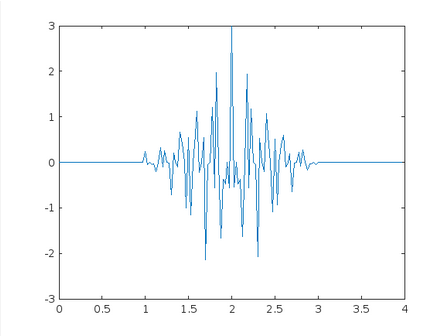
\includegraphics[width=8cm]{DSP1/r1_k2_3.png}
\end{center}
\caption{ハミング窓による切り出し結果}
\label{kukei_window}
\end{minipage}
\begin{minipage}{0.5\hsize}
\begin{center}
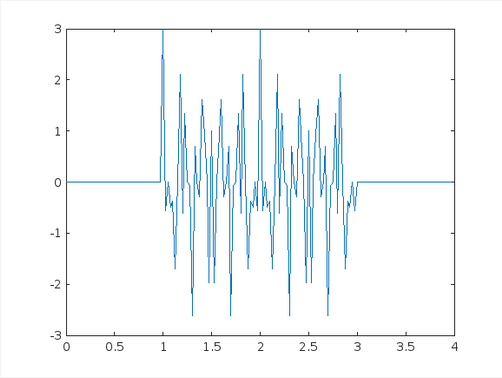
\includegraphics[width=8cm]{DSP1/R1_K2_6_kukei.png}
\end{center}
\caption{矩形窓による切り出し結果}
\label{hamming_window}
\end{minipage}
\end{tabular}
\end{center}
\end{figure}

図\ref{kukei_window}と図\ref{hamming_window}を比較すると、
矩形窓の切り出しでは波形をそのまま切り出していることもあり、波形、特に振幅の変化をとらえきれていない。
その一方でハミング窓の切り出しでは波形の振幅の変化をより正確にとらえている。

問題2-3:矩形窓とハミング窓による信号切り出し結果の振幅スペクトルを図示し
比較せよ。また各窓関数の結果の相違点について具体的に述べよ。

解答:
以下にハミング窓と矩形窓による切り出し結果の振幅スペクトルを示す。
%横に2枚の画像(jpg/png)表示
\begin{figure}[H]
\begin{center}
\begin{tabular}{c}
\begin{minipage}{0.5\hsize}
\begin{center}
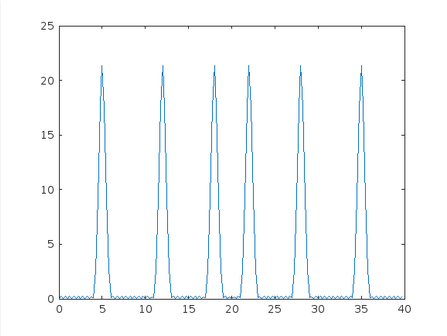
\includegraphics[width=8cm]{DSP1/r1_k2_4.png}
\end{center}
\caption{ハミング窓}
\label{hamming_spectol}
\end{minipage}
\begin{minipage}{0.5\hsize}
\begin{center}
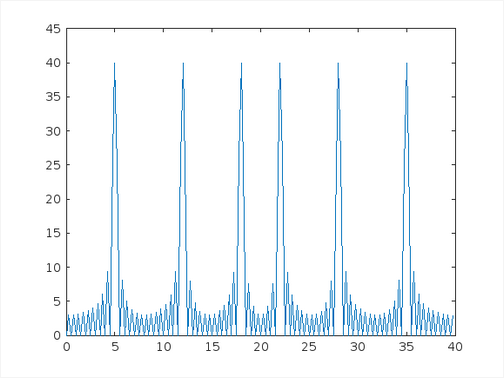
\includegraphics[width=8cm]{DSP1/R1_K2_7_kukei.png}
\end{center}
\caption{矩形窓}
\label{kukei_spectol}
\end{minipage}
\end{tabular}
\end{center}
\end{figure}

図\ref{hamming_spectol}と図\ref{kukei_spectol}を比較すると、
矩形窓での切り出し結果の振幅スペクトルの大きさは全体的に大きくピーク値は40、対してハミング窓での
切り出し結果は22程になっている。周波数のピーク値には特に違いは見られなかった。

また矩形窓のスペクトルのグラフはノイズを含んでおり、ハミング窓においてはスペクトルの波形が滑らかになっている。

応用課題:矩形窓とハミング窓それぞれの振幅スペクトルを図示せよ。また、その結果を考察せよ。

解答:
%横に2枚の画像(jpg/png)表示
\begin{figure}[H]
\begin{center}
\begin{tabular}{c}
\begin{minipage}{0.5\hsize}
\begin{center}
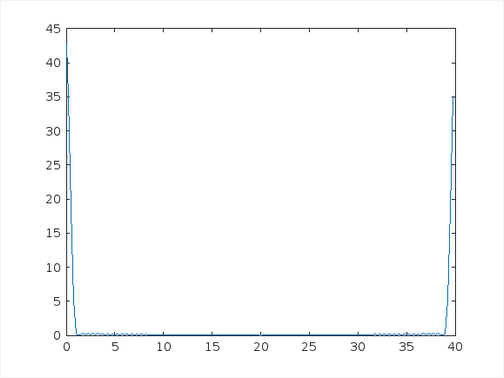
\includegraphics[width=7cm]{DSP1/R1_K2_8}
\end{center}
\caption{ハミング窓の振幅スペクトル}
\label{hammingcar_spectol}
\end{minipage}
\begin{minipage}{0.5\hsize}
\begin{center}
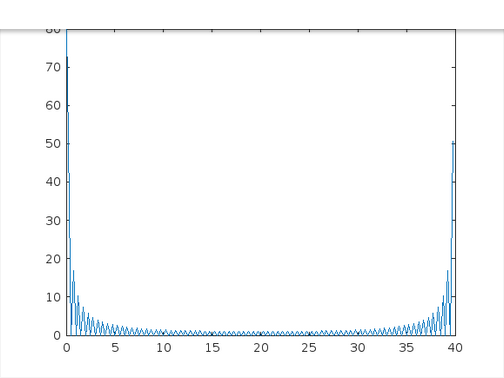
\includegraphics[width=7cm]{DSP1/R1_K2_9}
\end{center}
\caption{矩形窓の振幅スペクトル}
\label{boxcar_spectol}
\end{minipage}
\end{tabular}
\end{center}
\end{figure}

図\ref{hammingcar_spectol}と図\ref{boxcar_spectol}を比較すると、
ハミング窓の振幅スペクトルの最大値は40であり、ノイズは少ない。

一方で矩形窓の振幅スペクトルの最大値は70であり、比較的ノイズを多く含む。

よって矩形窓の切り出し結果にノイズを多く含んでいる、矩形窓の切り出し結果のほうが振幅スペクトルの値が大きいといった
特徴は矩形窓に起因している。

\section{考察}
実験の結果、高速フーリエ変換アルゴリズムと通常の離散フーリエ変換で得た値とでは若干の違いはあるものの
大差はないということが分かった。

ハミング窓と矩形窓とではハミング窓のほうが振幅の変化を忠実にとらえることができるといった観点から
サンプルデータの切り出し手法としてはハミング窓のほうが優れていると言える。
\section{感想}
今回の実験を通して、課題1を通してはMatlabの信号処理アルゴリズムはよくできているなという点を感じとった。
また信号処理の基本的な手法に触れたことで、信号処理の分野も面白い、Matlabをもう少し知りたいと感じた。

\begin{thebibliography}{9}
	\bibitem{Mat_official} MathWorks公式ドキュメント \url{https://jp.mathworks.com/help/matlab/ref/}
	\bibitem{class_ref} 信号処理Ⅰ 2024 講義資料
\end{thebibliography}

\end{document}